
\documentclass[journal]{IEEEtran}
\usepackage[utf8]{inputenc}
\usepackage{cite}
\usepackage[cmex10]{amsmath}
\interdisplaylinepenalty=2500
\usepackage{algorithmic}
\usepackage{array}
\usepackage{url}
\usepackage{mathtools}
\hyphenation{op-tical net-works semi-conduc-tor method methods}
\usepackage{float}


\ifCLASSOPTIONcompsoc
  \usepackage[caption=false,font=normalsize,labelfont=sf,textfont=sf]{subfig}
\else
  \usepackage[caption=false,font=footnotesize]{subfig}
\fi

\ifCLASSINFOpdf
  \usepackage[pdftex]{graphicx}
  % declare the path(s) where your graphic files are
  % \graphicspath{{../pdf/}{../jpeg/}}
  % and their extensions so you won't have to specify these with
  % every instance of \includegraphics
  \DeclareGraphicsExtensions{.pdf,.jpeg,.jpg,.png}
\else
  % or other class option (dvipsone, dvipdf, if not using dvips). graphicx
  % will default to the driver specified in the system graphics.cfg if no
  % driver is specified.
  \usepackage[dvips]{graphicx}
  % declare the path(s) where your graphic files are
  % \graphicspath{{../eps/}}
  % and their extensions so you won't have to specify these with
  % every instance of \includegraphics
  \DeclareGraphicsExtensions{.eps}
\fi

\floatstyle{ruled}
\newfloat{json}{thp}{lop}
\floatname{program}{Program}

%opening
\title{A Simulator for Event-oriented Data in Flexible Assembly System Fault Prediction - DRAFT}
\author{Tero Keski-Valkama}

\begin{document}

\maketitle
Version: \today

\begin{abstract}

\end{abstract}

\begin{IEEEkeywords}
\end{IEEEkeywords}

\section{Introduction}
This paper describes a method for simulating event-oriented data sources of a flexible assembly system (FAS) including faults. Such a simulator is required for creating representative corpuses
of data for teaching automated learning algorithms for predictive maintenance, condition monitoring and systemic fault detection.

Flexible assembly system was described by Donath and Graves \cite{donath1988flexible} as a collection of flexible assembly cells comprising one or several work stations connected by automatic material-handling devices.
In practise, a flexible assembly system contains parts and materials stored in an intermediate storage,
a conveyor or crane system to move the parts, materials, intermediate assemblies and finished products between the stations, and the stations with work machines and necessary tooling
to assemble, process or inspect intermediate assemblies and products. The stations might consist of for example manual assembly steps, and robotic assembly cells. In flexible manufacturing systems (FMS),
the work stations might contain more complex machining and manufacturing tools like CNC lathes, or 3D printing. FAS and FMS are considered interchangeable for the purposes of this article, although
they have different scheduling and configuration properties.
Often the assembly sequence has multiple ways of being executed for a finished product leading to some redundancy and more efficient scheduling in terms of utilization.

As opposed to more specialized industrial production systems, flexible assembly systems are designed for smaller batches and greater flexibility so that the set of end products can vary more widely.
For example, flexible assembly systems can be reconfigured more conveniently following the evolution of new versions of the end products. Flexibly assembly systems also allow for a wider range
of customization between the different end product instances of the same product. The nature of fast evolution of configurations and workflows, and heterogeneous operating conditions make
planning maintenance more challenging.

System downtime is a significant cost for flexible assembly systems. System downtime is reduced by preventive maintenance typically scheduled periodically.
Recently Internet of Things and opening of the networked industrial system APIs have created new possibilities for predictive maintenance and systemic fault detection. Different sites with similar
flexible automation systems have widely different environmental and workload conditions which has an impact on the wear and tear of the flexible automation system components.
Taking different site environments and workloads into account when planning preventive maintenance cycles is non-trivial. There is a clear need to adapt maintenance based on actual
conditions in the operation rather than by simply scheduling maintenance periodically\cite{hashemian2011state}.
It is also important to indicate potential faults early to improve the response time of corrective action.
Going from preventive maintenance towards predictive maintenance optimizes and targets the maintenance related costs towards the activities that have best impact
on improving the availability and operation of deployed flexible assembly systems.

Predictive maintenance in flexible assembly systems benefits from automatic indicators for immediate and potential future faults.
It is generally not possible to enumerate all the possible fault conditions and their sensory indicators of a flexible assembly system in an exhaustive fashion,
as the less common errors are forgotten and some faults might cause unexpected results\cite{camarinha1996integration}.
There is a need for autonomously learning systems which are able to deduce the correct operation of the flexible assembly system and report potential deviances. One way to monitor a process is to observe the symbolic
logs generated as the process is being executed.

Current predictive maintenance and condition monitoring systems concentrate on measuring device health for example by means of measuring temperature\cite{mobley2002introduction},
vibration\cite{scheffer2004practical}, lube oil particle analysis\cite{hunt1993handbook} and electrical current signals
\cite{thomson2001current}. Research on anomaly detection for non-interleaved discrete sequences is summarized in this survey\cite{chandola2012anomaly}.
Interleaved discrete sequences, or uncorrelated process traces have been mainly researched in relation to specification mining for multi-threaded or asynchronous software processes.
The solutions use domain-specific features to help in reconstructing the dependency graphs out of interleaved sequences. For example this solution works for message-oriented systems\cite{kumar2011mining},
and this solution requires sets of separate and complete traces corresponding to executions of an application\cite{mining-program-workflow-from-interleaved-traces}. Most process mining and specification mining
solutions aim to solve the challenging task of inferring a complete process model out of the logs, even if the interleaved logs themselves might exhibit some weaker form of features
and characteristics useful for anomaly detection.

Flexible assembly system process traces are not separable into complete and separate execution runs in the general case, because assembly process is typically continuous and
forms a single interleaved log with an arbitrary limiting window.
On the other hand, delays in processing steps are mostly independent of the whole system state, and could be hypothetically used to infer structure in the interleaved log.
There are also events unrelated to the processes, like timer ticks and analogous events. The main process events often follow stoichiometric laws in a normal operation corresponding to materials
not being created or destroyed within the process. Stoichiometric invariance is often clearly visible when drawing a histogram of event type counts in the logs showing that specific events corresponding to certain
assembly steps are done specific numbers of times per product, leading to counts of events for a specific event type strongly correlating with counts of other event types. If there are alternative routes of products
through the assembly process, the correlation is more specifically between sums of counts of alternative event type which might not be as easily visible.

Evaluating novel automatic methods for fault prediction requires standard benchmarks to compare these methods against. Currently there are no standard benchmarks to test
different symbolic log anomaly detection methods and compare their performance against each other. Such standard benchmarks exist in other fields of machine learning,
such as the MNIST handwritten digits benchmark\cite{lecun-mnisthandwrittendigit-2010}. Realistic simulations are often used\cite{jager2014assessing} for domains where
real data is hard to collect or where real data would be subject to business confidentiality. Training neural network and other learning systems often utilizes realistic
simulations instead of real data\cite{weston2014memory}. Real measured data is often limited in both state space and in volume,
and often simulations give better results \cite{duch2005artificial}.

Some simulations of flexible assembly systems are generally available\cite{giulio}\cite{el1989simulation}\cite{donath1988flexible} and have been studied for visualization and optimization purposes.
However, these are not directly suitable for benchmarking fault detection methods regarding interleaved discrete sequences.

\section{Problem Formulation}

A standard benchmark should reflect a realistic task and it should have enough representative data to be useful.

Real data regarding flexible assembly system faults is
not generally available, because fault data is generally subject to business confidentiality in flexible assembly industry.
The generally available simulation models do not typically contain failure modes and are not typically designed to emit
log structured events in a realistic fashion, but they can be used as a starting point in creating a flexible assembly system model.

To enable relevant research into anomaly detection in flexible assembly systems a realistic simulator for logged events is needed.
All references to simulated faults and failure modes in the research described in this article are hypothetical and should not be considered to
reflect actual characteristics of any specific existing systems. An effort is made to make the simulations contain the necessary features of
generic and realistic failure modes to make the models useful for research, but for example the simulated fault frequencies and the configuration
of the flexible assembly system along with workflows and end products are arbitrary and hypothetical.

A simulation for benchmarking anomaly and fault detection methods should not be fully deterministic to reflect the real world dynamics. The simulation should also
include realistic faults with possible early indicators such as variations in delays in the steps of the process. The focus of the simulator is on faults without pre-existing
diagnostic fault codes, such as unexpected faults and degradation of the assembly modules and conveyors, and on systemic faults. Systemic faults in this paper
are defined to mean faults and degradation of output where each of the component modules of the flexible assembly system are seemingly operating without faults. Execution failures
which are detected during execution of an action as a deviance of the state from the expected state are outside of the focus of this work, as these conditions are adequately detected and handled
by existing supervision systems.

\section{Modes of Failures in Flexible Assembly Systems}

Flexible assembly system failures are typically component failures where a failure of a single module or a component will lead to the part of the system becoming inoperational.
Since the flexible assembly systems are dynamic systems with numerous moving parts, the wear and tear of the components and tools are a significant source of faults.

In addition to the component failures, certain critical systemic failures can cause downtime, such as power loss and network communication failures.
The critical systemic failures mentioned don't typically show any indication before they happen so predictive maintenance has little potential to be applied there.
In addition to these critical system failures,
the whole system can exhibit modes of failure and degradation which are not directly attributable to single component degradation or failure.
Some of these might be caused by
external factors, such as accidents and human errors, but also for example by timing issues in the whole process causing unexpected queues or traffic jams.

Tool wear and tear depends on the workload. Typically tools that wear out fast, for example multiple times for one unit of work in a station, receive much attention and such tools are generally
well maintained. Tools that have wear and tear but have longer life spans are more susceptible to being overlooked by operators and might have some indicators of degrading
before a failure. Cranes, hatches and conveyors have relatively long life spans and are primarily maintained in periodic preventive maintenance. If we could get indicators
for impending failure for these components, the periodical maintenance could be scheduled earlier to prevent downtime.

In addition to these physical faults the flexible
assembly system can suffer from human errors. Human operator can inadvertently misconfigure the flexible assembly system so that its operating mode changes unexpectedly,
for example by disabling a station which can lead to the system stopping without a proper failure. In addition to configuration
errors, human operators might fail in manual assembly steps for example by pressing the button to mark the step
as completed too quickly.
The flexible assembly system might also get in incompatible materials, parts or replacement tools and fail when trying to use them.

There has lately been an increase of computer crime against industrial networks as the devices and systems become more connected.
Nation states execute industrial espionage and even sabotage against each other\cite{stuxnet}. An electronic sabotage attack might present itself
much like a human misconfiguration error, and would be potentially detected in a similar fashion even if the attack itself would not be
directly visible in the logs as anomalous activity.

Modelling the failure events can be based on Process Failure Mode and Effects Analysis (FMEA, PFMEA) \cite{teng1996failure} methodology which produces lists of
failure modes of components
in an assembly and machining process, and the respective effects of failures. For the purposes of learning systems it is not required that these failure modes and their frequencies
are perfectly realistic. However, the simulated failure modes should be expected to reasonably reflect the potentially detectable and anomalous failure modes of the process.
Ultimately, the learning system should model the correct operation of the system and detect deviances, rather than to learn specific failure modes.

For the purposes of describing the fault types we divide system components into slowly and
quickly degrading tools and auxilliary components. Tools are the components such as drill bits which are directly used to assemble or
machine the product. The auxilliary components are components with less expected wear and tear which are used to transport the products,
inspect the intermediate assemblies or dispense assembly components.

The fault types and distribution depend on the assembly system
and on the products being assembled. For one
specific assembly line \cite{cong1997fault} the common fault types were feeder errors, robot insertion errors,
robot grip errors, unqualified parts, fixture position errors, emergency stops, robot gripper collision,
grip sensor line break, and inspection equipment failures. The root causes for these are wear and tear, and incompatible parts.

For useful anomaly detection systems we need to concentrate on faults that are unexpected without pre-existing diagnostic error codes, and that potentially have early indications
in collected event-based logs. Early indication in this context means that the error can be detected in the system logs before the failure becomes otherwise evident.
The table \ref{faults} summarizes the classes of faults.

\begin{table}[!t]
\renewcommand{\arraystretch}{1.3}
\caption{Table of recognized fault types in flexible assembly systems}
\label{faults}
\centering
\begin{tabular}{|p{25mm}|p{15mm}|p{15mm}|p{15mm}|}
\hline
Fault type & Unexpected faults & Potentially has an early indication & Useful target for anomaly detection \\
\hline
\hline
Auxilliary component wear and tear & X & X & X \\
\hline
Station operation failures (feeder error, insertion error, grip error, fixture position errors) & & & \\
\hline
Critical systemic failures (power, network, emergency stop) & X & & \\
\hline
Human error, failed manual step & X & X & X \\
\hline
Incompatible parts, materials or replacement tools & X & & \\
\hline
Systemic failures (e.g. accidents and cyberattacks) & X & X & X \\
\hline
Tool wear and tear for quickly degrading tools (e.g. drill bits) & & X & \\
\hline
Tool wear and tear for slowly degrading tools (e.g. screwdriver) & X & X & X \\
\hline
\end{tabular}
\end{table}

\section{Flexible Assembly System Model}

The simulation consists of a realistic discrete event model of a flexible assembly system with a class of faults optionally injected into the process.
The initial simulation is very simple and does not incorporate complex scheduling and routing decisions or optimization like many flexible assembly/manufacturing system simulations\cite{donath1988flexible}.
However, it is a reasonable configuration of such a simple production system. More complex models can be implemented in the future.

Introducing synthetic faults into process data is a common method for testing whether the fault detection model works \cite{able2016model}.
Discrete Event Systems can be conveniently
described using Mixed Process Algebra Petri Nets (MPPN)\cite{falkman2001modeling}. In the following description we augment the MPPN with intervals between state transitions,
because event intervals are important information for deinterleaving the process traces.

Using the notation defined in \cite{falkman2001combined}, we note that the system can be described as an interleaved execution of $ n $ process instances $ P_i $, shown in
Equation \ref{interleaved_processes}.
\begin{equation}
 P_1 \oplus P_2 \oplus \textellipsis \oplus P_n
 \label{interleaved_processes}
\end{equation}

The interleaved process instances consist of sequences of $ m $ steps which are identical within a production batch in the simple assembly process being tested, shown in Equation \ref{identical_steps}.
More complex assembly processes might have several alternatives for specific steps, representing multiple interchangeable stations where an unit of work can be scheduled.
It is also possible for some processes that some assembly steps can be performed in an arbitrary order.
The sets B and U above the arrows denote the booking/unbooking sets constraining this transition, encapsulating the scheduling dependencies between process instances.
\begin{equation}
 P_i = a_1 \xrightarrow{B_2 \& U_1} a_2 \rightarrow \textellipsis \rightarrow a_m
 \label{identical_steps}
\end{equation}

Some steps are associated with exclusive resources which can be described by associating the transitions in the MPPN model with booking and unbooking resources, so that
the corresponding transitions in the general resource model Petri net shown in Figure \ref{figure:resource_model} trigger changes in the status of the resource and
are gated by the status of the resource.

\begin{figure}[tb]
 \centering
 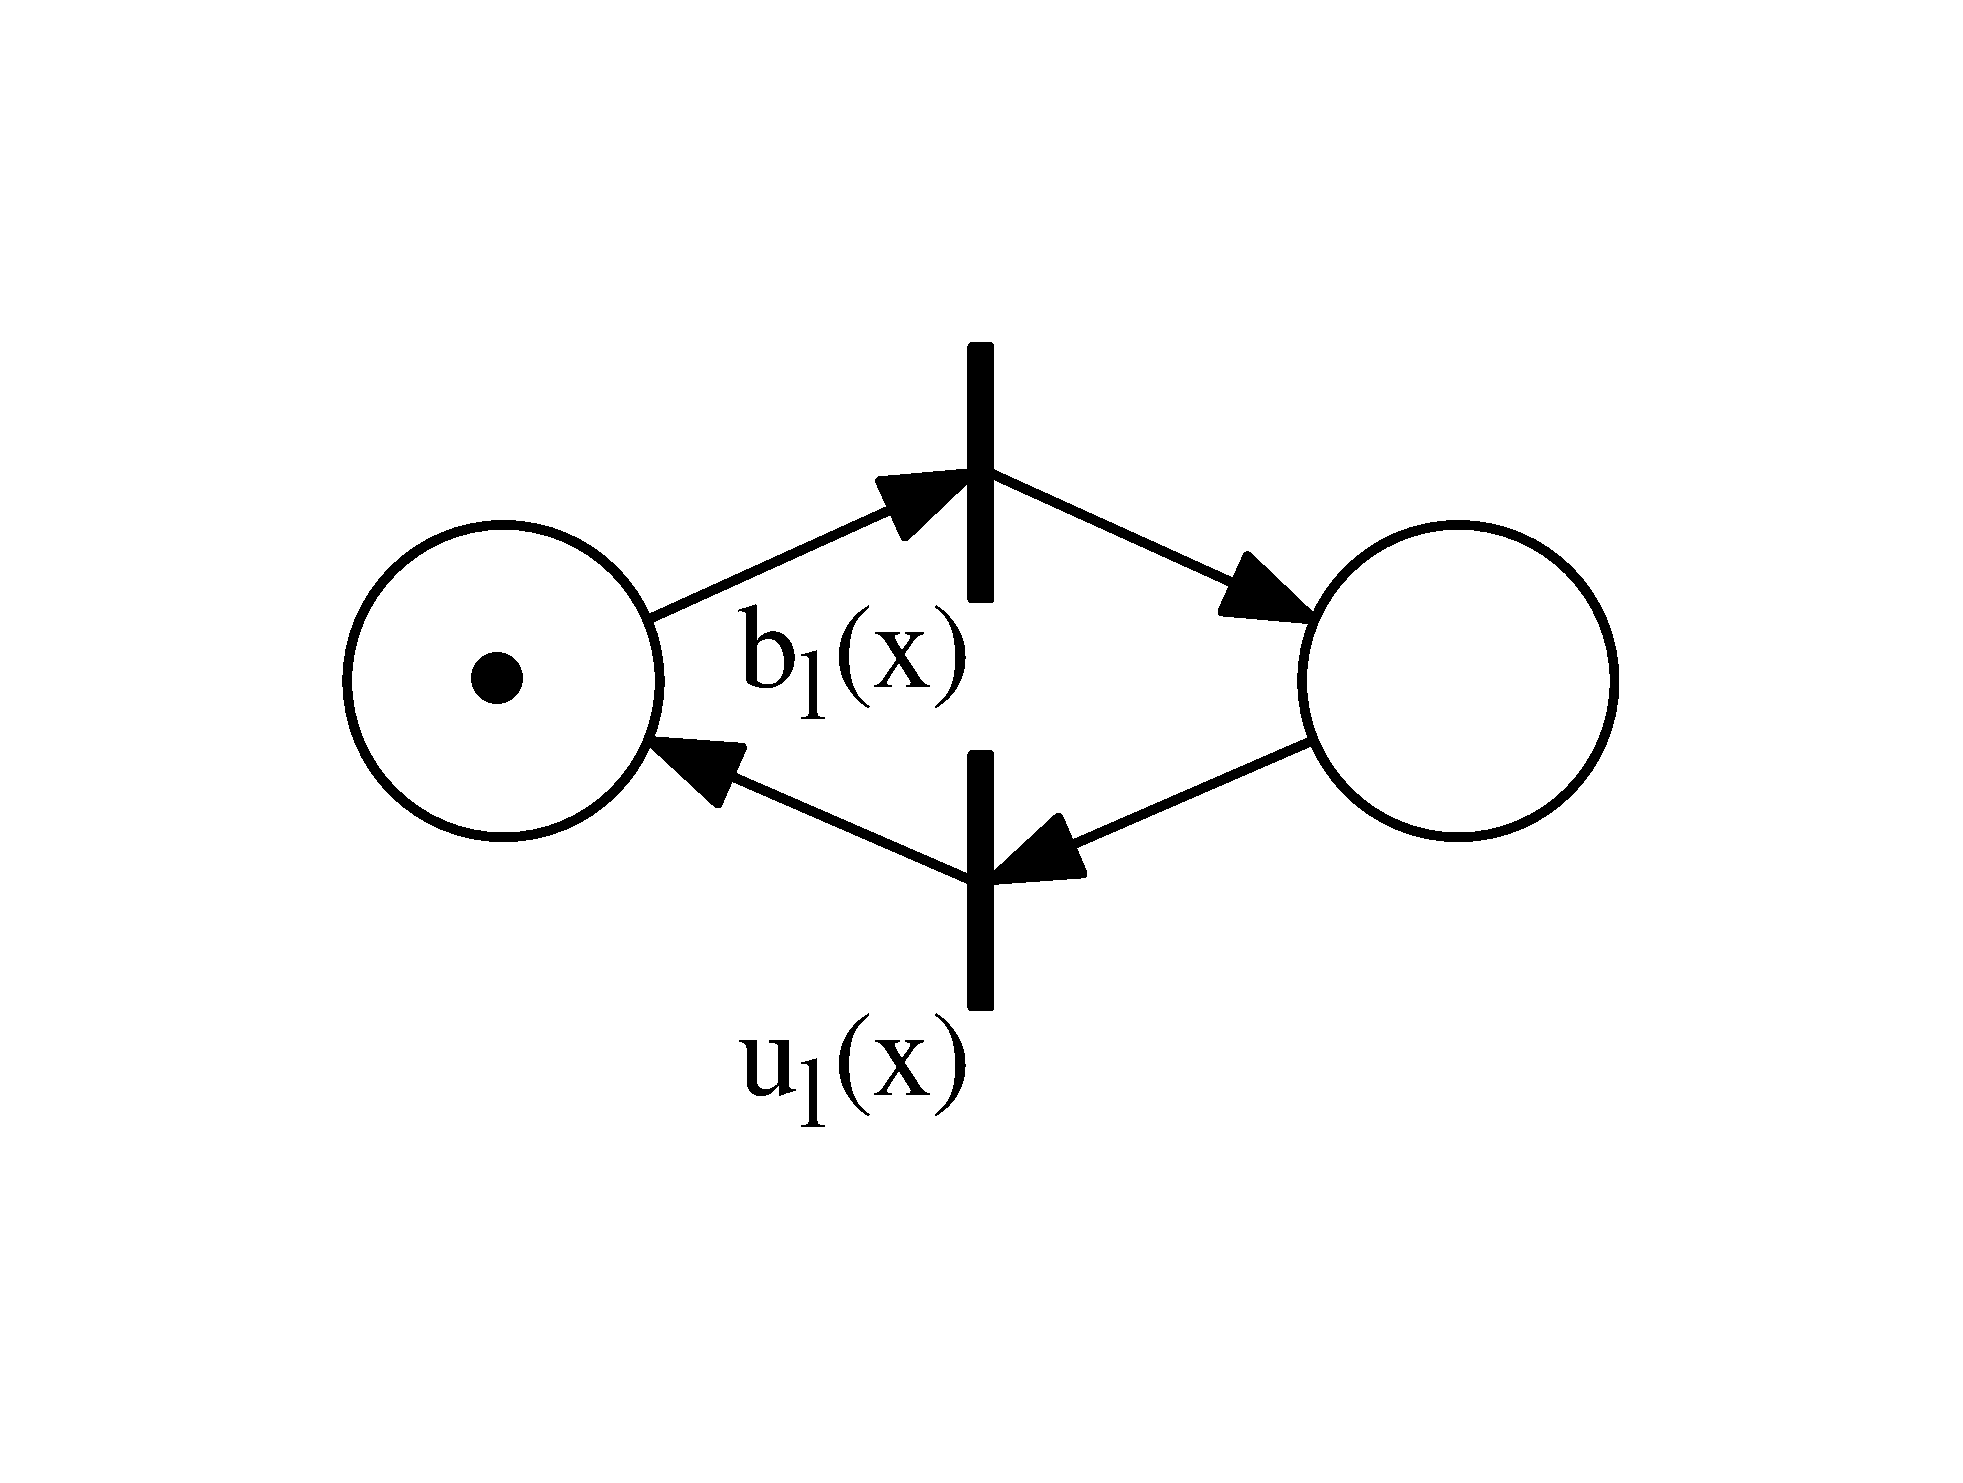
\includegraphics[width=8 cm,keepaspectratio=true]{./general_resource_model.eps}
 \caption{The general resource model Petri net showing resource booking and unbooking transitions for a single resource $ R_l $}
 \label{figure:resource_model}
\end{figure}

Symbolic process logs are generated by running the simulation. The event types form a flat, unstructured categorization. Hypothetically events could also be typed hierarchically or as a structured collection
of discrete features so that an event could be for example both
a trigger of a specific light gate, and a trigger of any light gate in general, being encoded in the logs as both the specific event type and the general one. The benefit of using a flat categorization is that
it can be trivially discovered from an existing system with minimal knowledge about the system by simply defining the mapping from log messages to a set of discrete log event types.
Depending on the target system being modelled, it might also make sense to encode the events as pairs of device id producing the event, and event type.

The simulation will not be fully deterministic and contains soft faults which do not affect operation in addition to hard faults which result in immediate downtime.
Flexible assembly system scheduling and production optimization is an active research field. Different scheduling models can be implemented into the simulation,
but the provided initial example is a simple sequence of mostly independent steps, as it roughly matches the studied Chrysler transmission assembly line.
Compared to modern flexible assembly systems, the Chrysler transmission assembly line is on the low complexity side of the spectrum, and incorporates a lot of manual steps.
Regardless, it is a good starting point for evaluating learning systems based on assembly log traces.

The simulator is implemented in Python using Simpy discrete event simulation library and it generates a JSON file which models the logs from the system.
The log message fields are defined in Table \ref{fields}.

\begin{table}[!t]
\renewcommand{\arraystretch}{1.3}
\caption{Log message fields}
\label{fields}
\centering
\begin{tabular}{|p{25mm}|p{45mm}|}
\hline
Field & Description \\
\hline
\hline
Timestamp & The time of the log message in milliseconds since the start of the simulation \\
\hline
Event type & A string identifier of the event type that also uniquely identifies the work step or the device notifying the event \\
\hline
\end{tabular}
\end{table}

The simulation framework consists of a scheduler that takes the next event from the event queue and applies it to the respective module. The simulated modules
execute when events are applied to them and generate new events and immediate log entries with timestamps and other metadata.
The simulated modules have optional active failure modes that affect the simulated operation of the component through
generated log messages or the subsequent generated events. Failure modes are set up to the simulated modules in a separate failure module.
The overall framework sets up the simulation, that is the configuration of the process, bootstrap events and optional failures.

\subsection{Normal Operation of the Simulated System}
The simulated hypothetical system assembles and tools a car transmission block loosely inspired by a Youtube video of Chrysler transmission assembly\cite{transmission}.
The workflow consists of several manual assembly steps in separate stations and transporting the subassemblies between the stations by the means of
cranes and conveyors. Combining separately assembled subassemblies is a common activity in flexible assembly systems\cite{el1989simulation}.
Multiple transmission blocks are being assembled simultaneously in separate, independent stations.

The transmission component consists of four subassemblies. The main sequence starts from the frame of the transmission block
and continues through several manual steps done in separate stations. The steps of the main sequence are given in
the Tables \ref{mainsteps1} and \ref{mainsteps2}.
Each step contains a separate sequence of events and associated log messages defined in the tables. The log messages include the component which logged the event, but
not the process instance.
The durations vary in normal distribution. The durations for manual steps in normal operation have a standard deviation of five percent of the mean. The durations for automatic steps
have a standard deviation of one percent of the mean. Durations are clipped to be non-negative.

The production frequency of the transmission blocks depends on the slowest step as in this case there is only one station for one step and no
parallel work is possible within one station. The slowest step takes about 76 seconds. In this hypothetical assembly plant, new transmission block
frames are added every 100 seconds and the final transmission blocks are being produced roughly in the same interval. This means that there
will be at maximum roughly seven transmission blocks in different stages being produced at the same time.

\begin{table}[!t]
\renewcommand{\arraystretch}{1.3}
\caption{Table of the steps 1-16 in the main assembly process}
\label{mainsteps1}
\centering
\begin{tabular}{|p{5mm}|p{20mm}|p{10mm}|p{15mm}|p{15mm}|}
\hline
Step & Description & Duration & Log messages \\
\hline
\hline
1 & Crane & 30 s & Going forward, stopping, going back, stopping \\
\hline
2 & Manual inspection & 37 s & OK pressed, queue alarm \\
\hline
3 & Conveyor & 30 s & To station, stop, to next station \\
\hline
4 & Bowl feeder gives components & 5 s & Given \\
\hline
5 & Add components & 21 s & OK pressed, queue alarm \\
\hline
6 & Conveyor & 30 s & To station, stop, to next station \\
\hline
7 & Bowl feeder gives components & 10 s & Given \\
\hline
8 & Add components & 34 s & OK pressed, queue alarm \\
\hline
9 & Conveyor & 30 s & To station, stop, to next station \\
\hline
10 & Crane with subassembly A & 10 s & Going forward, stopping, going back, stopping \\
\hline
11 & Combine with subassembly A & 34 s & OK pressed, queue alarm \\
\hline
12 & Conveyor & 30 s & To station, stop, to next station \\
\hline
13 & Conveyor with subassembly B & 10 s & To station, stop \\
\hline
14 & Combine with subassembly B & 35 s & OK pressed, queue alarm \\
\hline
15 & Conveyor & 30 s & To station, stop, to next station \\
\hline
16 & Bowl feeder gives components & 5 s & Given \\
\hline
\end{tabular}
\end{table}

\begin{table}[!t]
\renewcommand{\arraystretch}{1.3}
\caption{Table of the steps 17-31 in the main assembly process}
\label{mainsteps2}
\centering
\begin{tabular}{|p{5mm}|p{20mm}|p{10mm}|p{15mm}|p{15mm}|}
\hline
Step & Description & Duration & Log messages \\
\hline
\hline
17 & Conveyor with cover & 10 s & To station, stop \\
\hline
18 & Add cover and bolts & 76 s & OK pressed, queue alarm \\
\hline
19 & Conveyor & 30 s & To station, stop, to next station \\
\hline
20 & Tighten the bolts & 28 s & OK pressed, queue alarm \\
\hline
21 & Conveyor & 30 s & To station, stop, to next station \\
\hline
22 & Conveyor with subassembly C & 10 s & To station, stop \\
\hline
23 & Combine with subassembly C & 60 s & OK pressed, queue alarm \\
\hline
24 & Conveyor & 21 s & To station, stop, to next station \\
\hline
25 & Tighten the bolts & 16 s & OK pressed, queue alarm \\
\hline
26 & Conveyor & 21 s & To station, stop, to next station \\
\hline
27 & Bowl feeder gives components & 5 s & Given \\
\hline
28 & Add components & 11 s & OK pressed, queue alarm \\
\hline
29 & Conveyor & 21 s & To station, stop, to next station \\
\hline
30 & Tighten the bolts & 32 s & OK pressed, queue alarm \\
\hline
31 & Conveyor & 21 s & To output gate \\
\hline
\end{tabular}
\end{table}

\subsection{Simulated Failure Modes}
It is regrettable that real data on fault modes in real flexible assembly systems is not publicly available, but in any case it is possible to make reasonable
models based on existing data from other analogous sources such as \cite{nasaames} and \cite{tsarouhas2009classification}. Specialized simulations designed
to reflect specific assembly line conditions can be based on process FMEA reports. In the example described in this article, the fault modes are arbitrary, but 
can be reasonably expected to roughly reflect real conditions.

The previous subsection describes the normal operation of the system. The failure modes of the manual steps include human errors by pressing an OK button
signifying a completed manual assembly step prematurely without properly executing the step. This leads to the next manual step failing and
returning the block back to the previous step or removing it from the assembly line altogether.
Failed manual steps also include wear and tear
on the tools which gradually increases the duration of the work before causing a fault. The human operator can also tire and lose concentration
when doing lots of repetitive steps. There are studies showing how speed performance degrades in general in a linear fashion in humans
under fatigue and boredom, for example \cite{fatigue}. Switching human operators during the day might change the effective performance slightly.

The automatic steps wear and tear cause gradually increasing durations for the step also until at some point the step stops functioning and
intermediate assemblies start piling up until a fault is signalled because of exceeding the limits of intermediate storage space.

Duration increases before a fault are non-deterministic and for some faults they don't actually happen before the fault. The profile of the duration
increase depends on the type of device used for the step. Generally mechanical wear and tear effect on machine health profile follows
an accelerating curve downwards \cite{eker2012major}, \cite{milldataset}. For the purposes of simulation we can assume machine health has an approximately
linear effect on machine performance measured in delays and success rates in applicable types of faults.

Simulated wear and tear causes two types of delay profiles. First,
a continuous wear and tear typically causes no measurable delays at first, but when the degradation accumulates the delay increases following
a roughly exponential curve shown in the Figure \ref{figure:continuouswearandtear}. Second, for certain steps, such as taking bolts from the bowl feeder a human operator
might fail to grab a bolt from time to time. Typically the human operator tries again until successful. The frequency of the failure increases
slowly and roughly following an exponential curve until the failure rate becomes apparent and causes the operator to take corrective action,
typically causing downtime. These failures cause a random delay if they happen. This characteristic delay profile is depicted in the Figure \ref{figure:retrydelays}.

\begin{figure}[tb]
 \centering
 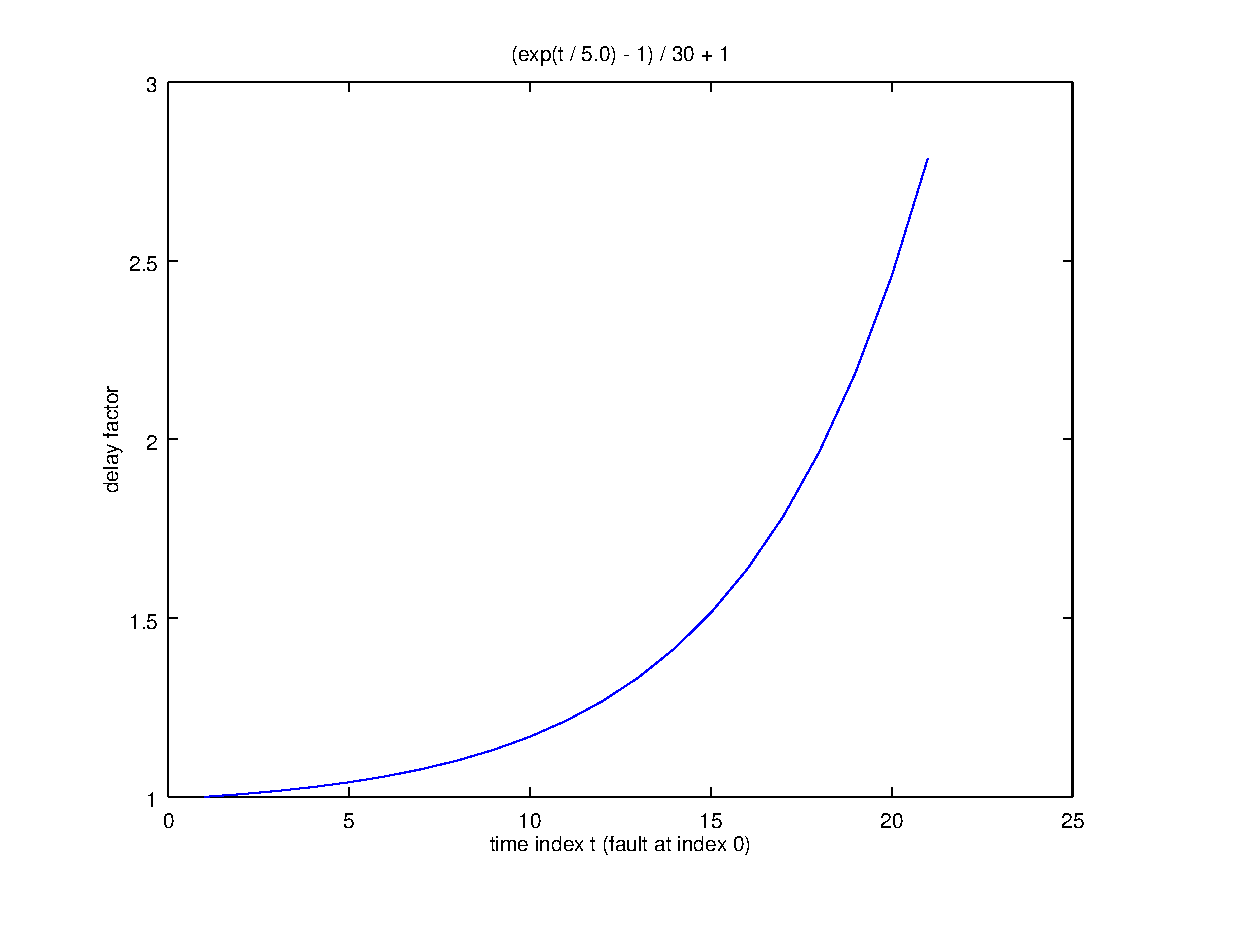
\includegraphics[width=8 cm,keepaspectratio=true]{./failure_profile.eps}
 \caption{A delay profile of continuous wear and tear}
 \label{figure:continuouswearandtear}
\end{figure}

\begin{figure}[tb]
 \centering
 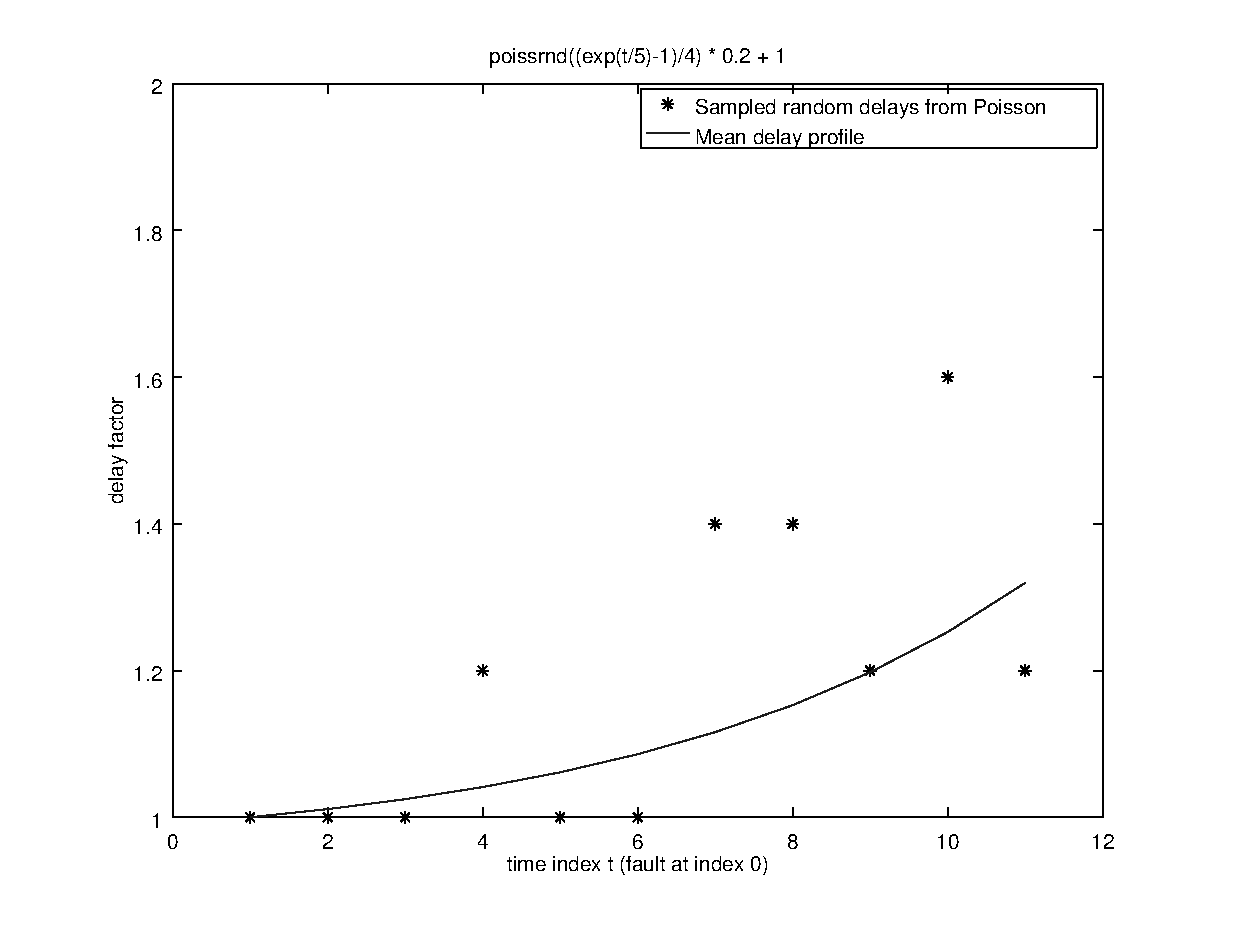
\includegraphics[width=8 cm,keepaspectratio=true]{./retry_profile.eps}
 \caption{A characteristic delay profile of human operator retry delays}
 \label{figure:retrydelays}
\end{figure}

A misconfiguration can cause different kinds of results. It is possible for example to choose an incorrect version of a Numerical Control (NC) program for a machining cell. It is also possible to
misconfigure the required steps for a final product. Here we assume that some work step is skipped
so that it is not noticed and doesn't directly prevent the subsequent steps from being executed. As the assembly process works exactly as configured, a traditional fault detection system comparing
the events to the configured process would miss this kind of a problem.

When there are human operators or assembly line workers in the assembly process, there are always human errors and accidents. For the purposes of this simulation we
assume a specific assembly worker has become incapacitated for a medical reason. This is a good target for anomaly detection, because sometimes there is no specific fault code
triggered if the human operator stops performing the assembly step.

Cyberattacks are becoming more frequent in the industrial domain. Both Stuxnet and BlackEnergy have been developed to specifically target SCADA industrial control systems.
These malware frameworks are modular with switchable components for different vectors, different targets and different functions.
In practice, these have been used for industrial espionage and sabotage. For the purposes of this article, only sabotage is considered.

There are at least two methods for how these kinds of malware can affect the industrial operations
after successfully penetrating such facilities. One, the control computer systems are destroyed by wiping the disks and shutting them down. BlackEnergy malware
successfully shutdown an Ukrainian Prykarpattyaoblenergo electric utility in Ivano-Frankivsk Oblask with this mechanism in 2015 December 23th.
Two, a tailored attack is implemented, so that specific physical vulnerabilities are abused in the plant systems. Stuxnet allegedly used a special function
to affect uranium enrichment centrifuges in Iran’s Natanz nuclear facility in 2010 in a subtle way causing the centrifuges to tear themselves apart.

This kind of sabotage is a good target for anomaly detection, because the effects and failures they cause are unexpected and it is possible that the primary control systems
have been disabled so they are incapable of handling faults in the normal way. For this example simulation, we disable the Crane with subassembly A by flooding it with commands
to repeatedly transport it to the other end position. The hypothetical attacker assumes this causes the system to jam up as the products are not being transported to the next
assembly stations. The attacker also assumes that this does not trigger a fault code as the crane is technically functioning perfectly.

While the directly visible fault modes are easier to model and characterise, complex flexible assembly systems also have warnings and trace messages
which are signalled into logs, but are not signalled to operators in real time because most of the time these messages are not a cause for concern.
An example of such a signal could be for example a health warning of a device that happens spuriously once every now and then for normal operation,
but increases in frequency when the device actually starts to fail. There can also be log messages for example for electrical switches turning
on and off when the working step is active, but never while the step is not active. Anomalies in such messages can be indicators of potential
future faults.

The simulated failures and their effects are listed in the table \ref{failures}.
To have a meaningful simulation of a system under faults we only need to simulate some representative fault conditions.

\begin{table}[!t]
\renewcommand{\arraystretch}{1.3}
\caption{Table of the simulated failures}
\label{failures}
\centering
\begin{tabular}{|p{20mm}|p{20mm}|p{20mm}|}
\hline
Failure & Description & Effect \\
\hline
\hline
Failed manual step & The human operator tries again until successful & A poisson distribution of delay for the step 7 \\
\hline
Wear \& tear & The completion time for the step degrades & The delay for the step 20 is exponential \\
\hline
Misconfiguration & The process is misconfigured & Steps 19 and 20 are skipped, process continues otherwise normally \\
\hline
Accident & A human assembly worker becomes incapacitated for a medical reason & Step 14: Combine with subassembly B stops \\
\hline
Cyberattack & An attacker disables a crane by flooding it with commands  & Step 10: The Crane with subassembly A is repeatedly moving to end position without transporting the subassembly A \\
\hline
\end{tabular}
\end{table}

\section{Implementation}

The FAS Simulator\cite{FASSimulator} is implemented in Python as a discrete event simulator using Simpy discrete event simulation library.
Each step of the assembly process is a Simpy resource and a process which receives and generates
delayed events in model time. Each step of the assembly process manages its own internal state, and possible failure modes.

The example simulation consists of stereotypical models of the steps of the process with input signals and configurable output signals. For example, simulating
the operation of a crane an instance of a module named Crane is configured and added to the respective position in the process in relation to other module instances.
The Crane module has a capacity of one item to transport at a time, and generates delayed output events for each of the input event in sequence, so that only one item is
transported at a time. This is in contrast to conveyor module instances which don't have a limited capacity, as the conveyors transport the items independently and in parallel.

The simulation is set up by first defining the all the modules in the assembly plant, and then the sequence of the activities by defining the process. The actual simulation
is done simply by triggering the global process inputs as required, causing sequences of events being generated accordingly. For interleaved process traces we instantiate multiple
parallel processes that share the resources in the simulated assembly plant.

The events are logged in JSON with a timestamp and an event type, resembling logs in a real flexible assembly system. The logs are not exported to
Mining eXtensible Markup Language (MXML) format, because MXML requires that separate process instances are identified. It is possible to make statistics of the internal simulator
state, for example graphing the queues forming at different points of the assembly plant. However, for the purposes of learning system development, the generated log output is the most
interesting resulting artifact.

The simulator in principle allows defining different kinds of discrete event simulations. Several specific types of simulations are pre-defined for the purposes of benchmarking
different modelling approaches. These pre-defined simulations vary in complexity and length from trivial one item at a time sequences to complex multiple items at once simulations.
Each type of simulation can also be configured to fail in specific ways to test different failure detection approaches. All the simulations are based on the flexible assembly system
defined in this article and the simulations are stochastic in respect to delays between steps.

In addition to the events related to specific process traces, we will add an event for an alarm if the queue waiting for a manual process is larger than five items. Also, we will
add a periodical ``tick'' event for every 10 seconds to allow for the learning system a realistic way of perceiving time, but also to include events that are unrelated to
the processes being executed, to reflect real logs. One conveyor is reused for two process steps, the steps 6 and 9. This means that these conveyor events
trigger twice for each product. This is to demonstrate a common situation where there might be multiple identical events of a specific type
associated to a single process trace.

\section{Mathematical Description}

Mathematically, the logs generated by the FAS Simulator can be described as a set of largely independent sequences each describing a successful assembly of one product instance shuffled, or interleaved
together.
For simplicity we consider only sequences where the assembly line is run successfully from empty start state to empty end state without modelling delays and queues, even if those are modelled in the underlying
simulation.
A formal language that accepts such sequences is called shuffled language \cite{berglund2011recognizing}. These languages are context-sensitive, so modelling methods
relating to regular and context-free languages are inadequate. For example Langer et al. \cite{langer2011self} showed that Angluin learner was able to learn small
toy examples very well, but didn't work very well for a real world example of a stream of events recorded from a CAN bus of the powertrain network of an electric vehicle.

FAS processes are often modelled as colored Petri nets \cite{saitou2002robust}, which require that the process instances are known for log messages
In practice, the process instances for log messages can only be known in the process
if the process is at least implicitly known in advance. For the general case we do not know which events correspond to which process instances, and some systemic events
in fact might affect multiple process instances at once. As in this
case process instances are not known, and all events are interleaved together for each process instance running concurrently, the most appropriate formal
model in the analysis time would be a Petri Net.

Automatic deinterleaving the logs and deducing the process instances for the log messages would simplify the model generators and models required
for evaluating the allowed sequences.
For example, if the log events contained the identifier of the product
item under the assembly step, anomaly detection would be much easier but such detection algorithms would not generalize as well
to new environments where such information is not available. Additionally, any system that assumes specific structure in the logs, for example that each event corresponds to
only one specific process instance, would likely fail in real world systems where these assumptions don't apply.

\section{Practical Evaluation}

The simulation is considered useful if it can be reasonably expected to mirror the real world contingencies and patterns, and if it is not completely trivial to
learn or infer by existing methods. If the simulator creates event sequences that are challenging to learn by existing methods, then it is useful as a benchmark
in relation to improving those methods and in creating new ones.

For the purposes of this article, we will only consider methods which are not trained based on known error conditions beforehand. Thus, the failure prediction challenge
becomes a challenge of learning the correct operation of the system and flagging any inconsistencies and anomalies.

For evaluation purposes, we will use a generated fault-free event sequence with first one complete sequence for one item only, then for 30 items simultaneously going through
the system simultaneously in the same log file. This results in a log file with a sequence of 1364 events of 36 different
event types. A depiction of the simulated event sequence is shown in the Figure \ref{figure:events}. The tick event is prominent in the bottom.
The first item goes through the process alone, so the events on the left side
of the graph are in a deterministic order from the bottom to the top. However, for multiple parallel items being processed it becomes evident that the previous event doesn't in itself
completely determine the next event.
Some queue effects are also visible in the later parts of the sequences showing the queue alarm event at the top and resultant cumulative delay for the event index 22.

For evaluating whether there is enough information in the sequence to determine some structure in the model, the sequence was visualized as grayscale pixels in Figure \ref{figure:output_easy}.
If human eye can make out some structure in the sequence, then in principle it is possible for the automated algorithms to do so also. To assist the eye, the pixel colors are chosen
from an ordered grayscale map, and the states are indexed in the order they are met in the log. It is possible to discern the three different length production batches from the image.
For each batch there are
a number of products assembled which corresponds to the same number of certain production related events, although that is not immediately clear for human eye.
For comparison, Figure \ref{figure:output_easy_wear_and_tear} was
created for situation where a simulated wear and tear fault happens in one of the conveyors, slowing its operation down slightly. Comparing the two simulations visually it is evident that the second process
is slower in the end of the batch, featuring tick events in longer sequences.
Similarly a retry delay fault with the bowl feeder can be seen in the Figure \ref{figure:output_easy_retry_delay}. As the retry delay affects a process step that is relatively fast, and does not 
represent a bottleneck in the process, it does not have a significant impact to the process.

It should be noted that while this kind of wear and tear fault would also be evident from measuring the process throughput, process throughput is a function of many other variables as well,
so in itself it is not an adequate measure of faults. A general anomaly detection system only observing event logs does not necessarily have a complete process model, but
can still observe these kinds of deviations from expected kind of activity.

Sonification is an audio display method where data is represented as non-verbal sounds. A sonification of the event log generated with timestamps and delays taken into account
is available here\cite{PHONOZATION}. Delays bring new features into the model, and
we can immediately note that certain events happen practically simultaneously (as multiple log lines are generated at the same event). Also, slower tempo tells us that less is
going on in the assembly line, and this could in principle give us a baseline for decomposing the canon-like interleaving of separate process instances from the whole.
If a human test subject can discern between the proper operation of the assembly line from random, or anomalous operation by the event log sounds,
then a machine could in principle be able to learn to do so also from the raw logs. It should be noted that this is not simply an exercise of deinterlacing interlaced events, because
the process traces do have interaction through limited process resources, which presents for example as saturations in bottlenecks.

We know that material balance requires that each log event strictly associated to a later part of process requires the number of requisite steps before it can be executed, and
therefore the associated log events must be present. Analogously this relates to the principles of stoichiometry and material balance used in chemistry and industrial processes.
For such a simple process what we have used as an example, most events occurs once and only once for each process instance, so drawing a histogram over a time window of a logged
composed of such process traces forms an equal distribution, discounting window effects.

\begin{figure}[tb]
 \centering
 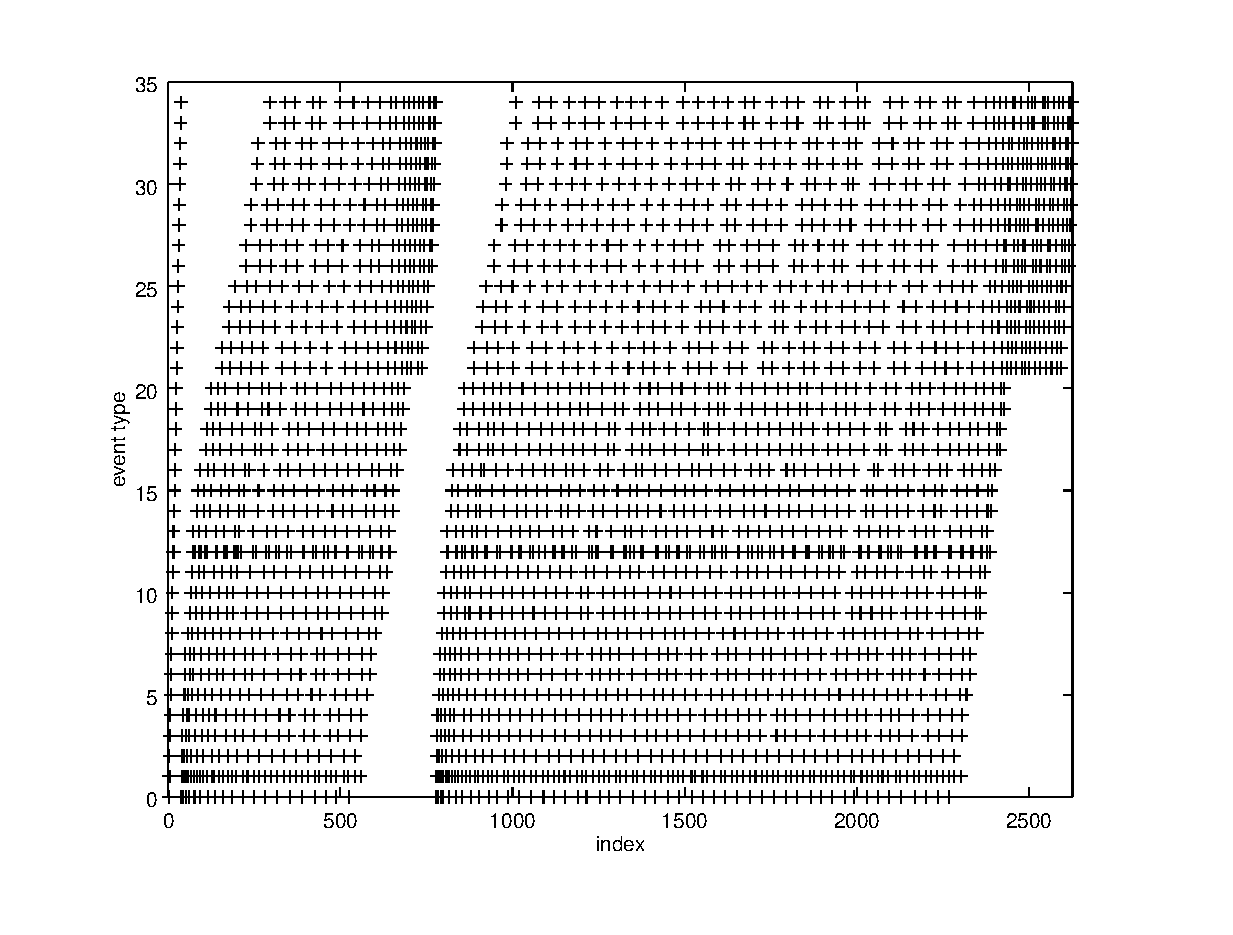
\includegraphics[width=8 cm,keepaspectratio=true]{./representative_log.eps}
 \caption{A representative log of event types graphed against time index}
 \label{figure:events}
\end{figure}

\begin{figure}[tb]
 \centering
 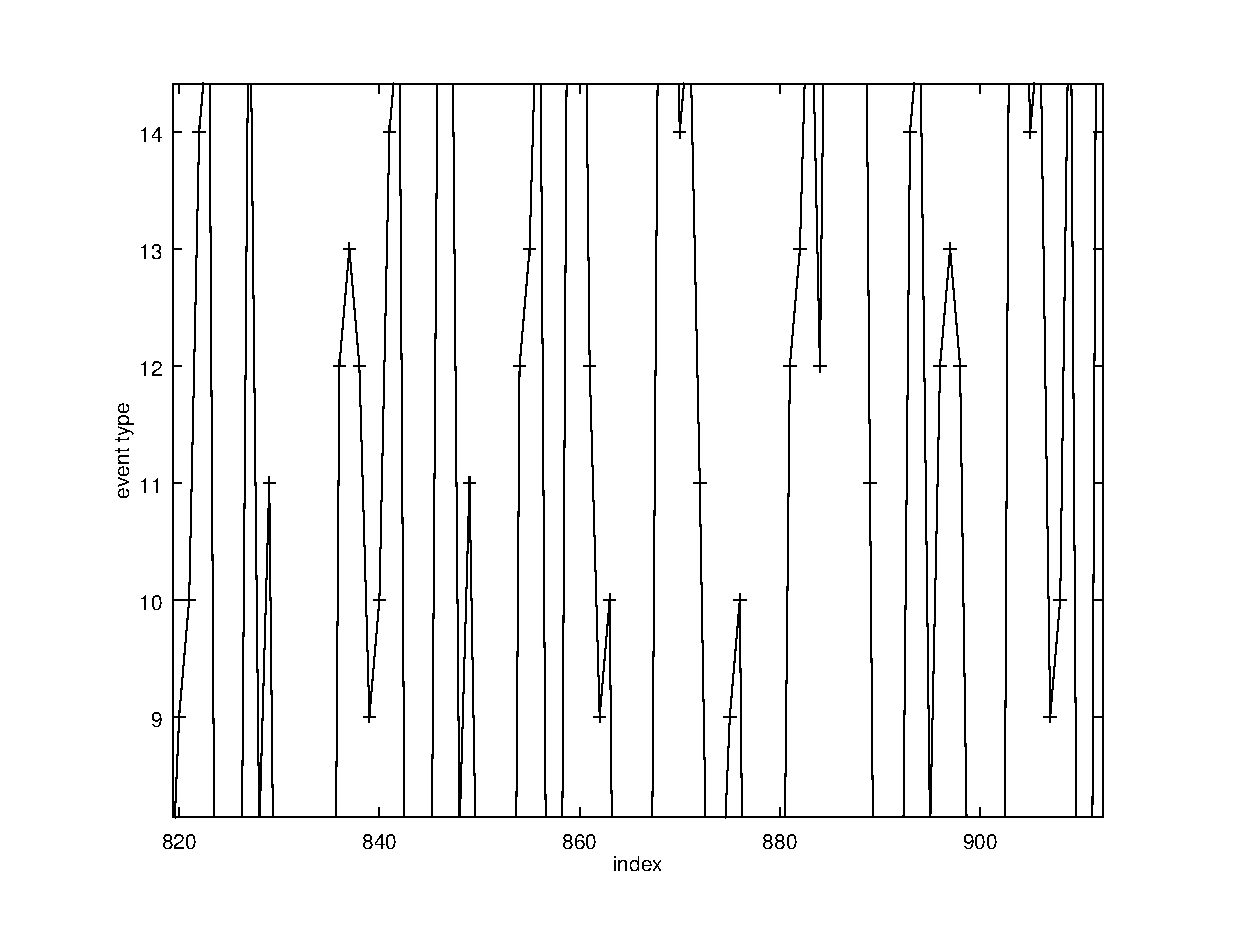
\includegraphics[width=8 cm,keepaspectratio=true]{./detail.eps}
 \caption{A detail of the graphed log of events. The lines connect the events in sequence, showing the indeterministic order}
 \label{figure:zoomed_events}
\end{figure}

\begin{figure}[tb]
 \centering
 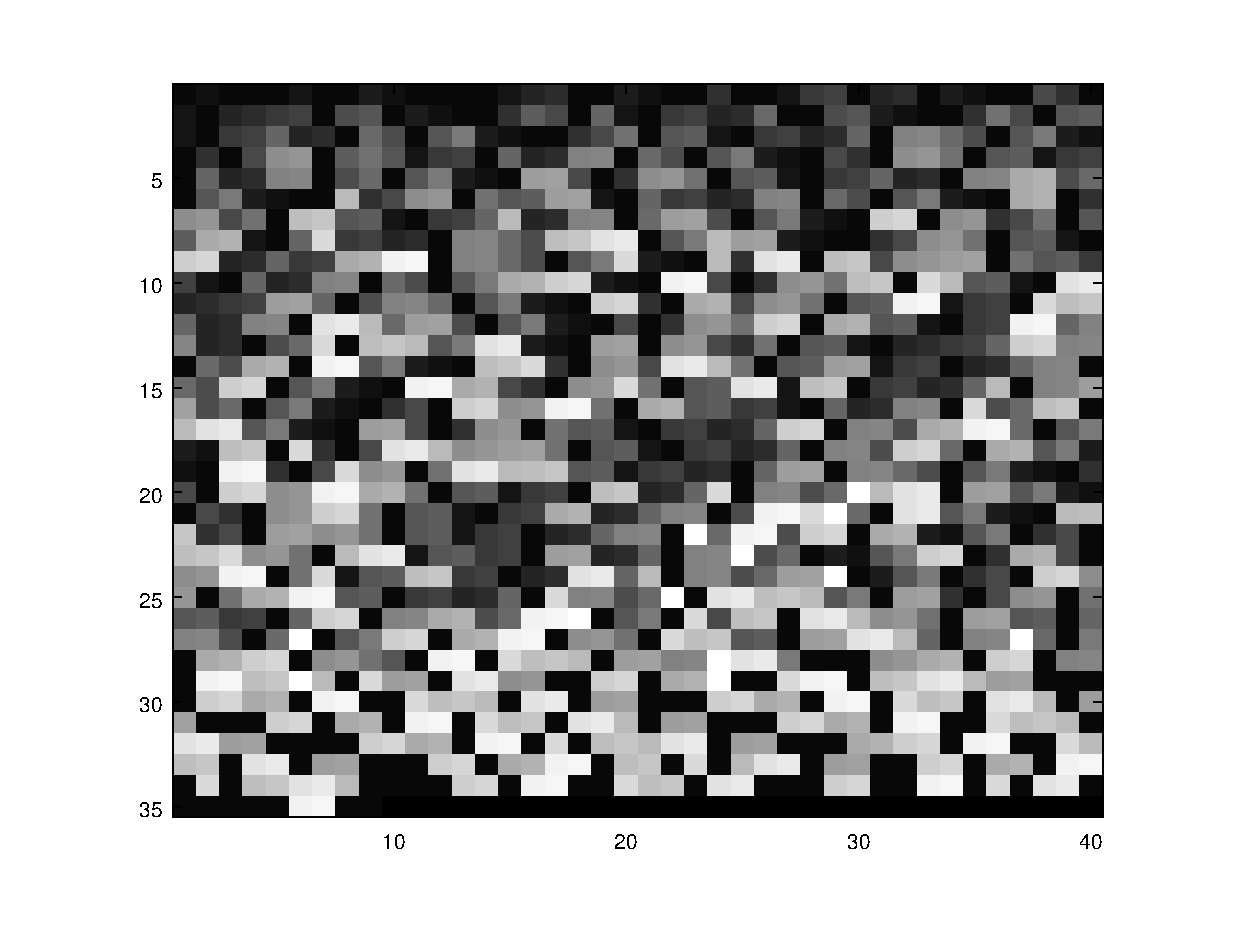
\includegraphics[width=8 cm,keepaspectratio=true]{./output_easy.eps}
 \caption{The event sequence as grayscale pixels from left to right, top to bottom, padded in the end with zeros.}
 \label{figure:output_easy}
\end{figure}

\begin{figure}[tb]
 \centering
 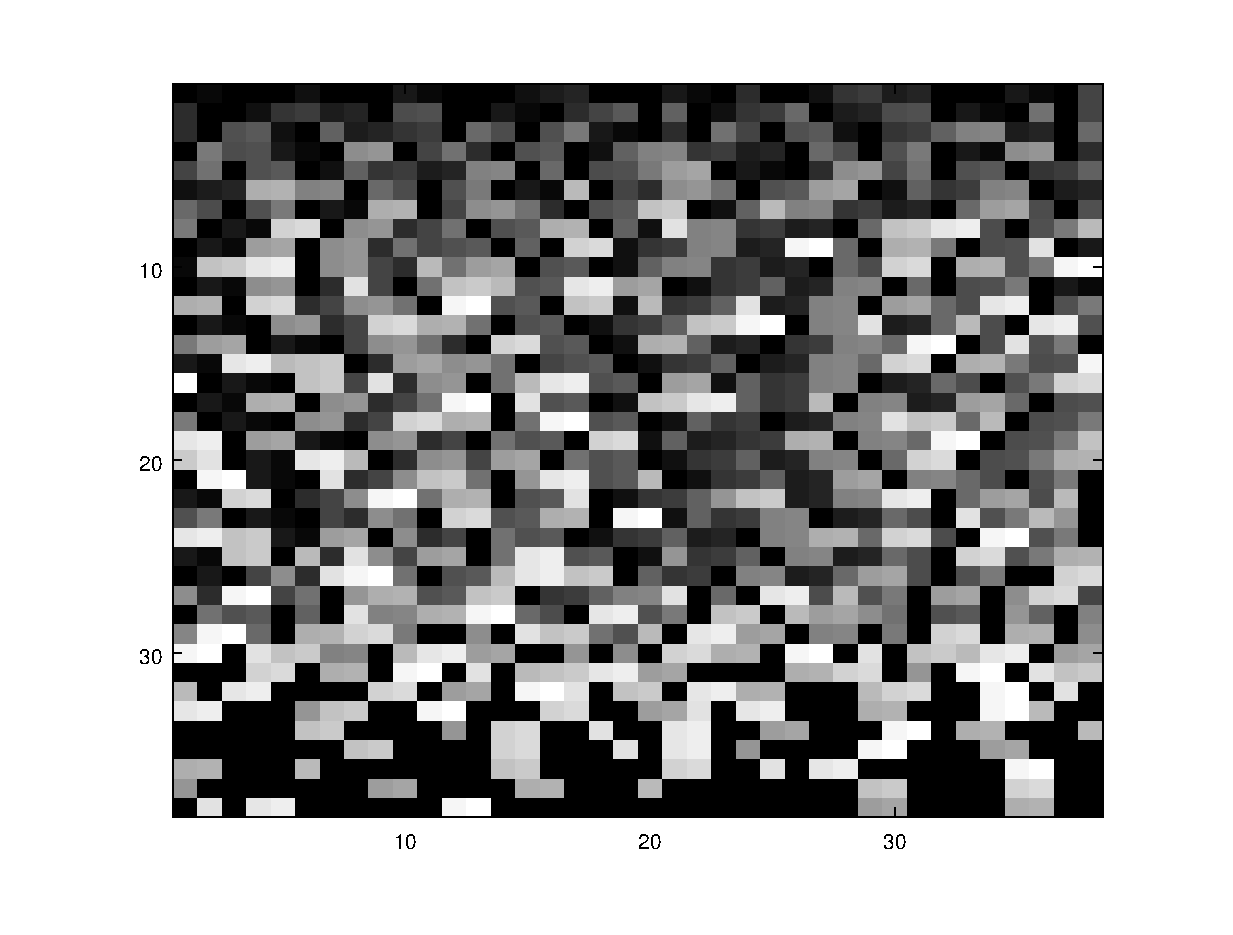
\includegraphics[width=8 cm,keepaspectratio=true]{./output_easy_with_wear_and_tear_fault.eps}
 \caption{Same as previous, but with a simulated wear and tear fault in step 15 conveyor.}
 \label{figure:output_easy_wear_and_tear}
\end{figure}

\begin{figure}[tb]
 \centering
 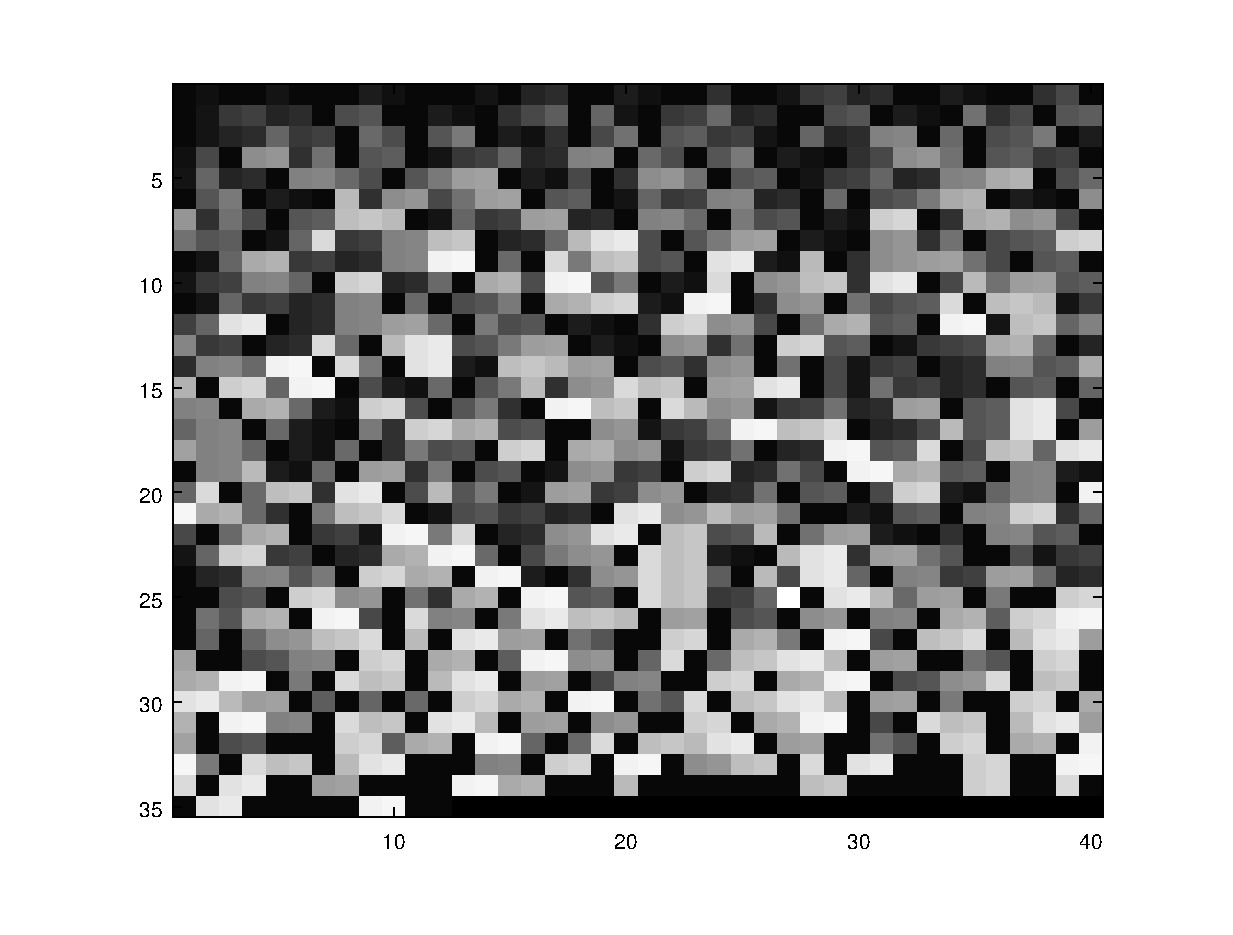
\includegraphics[width=8 cm,keepaspectratio=true]{./output_easy_with_retry_delay_fault.eps}
 \caption{Same as Figure \ref{figure:output_easy}, but with a simulated retry delay fault in step 7 bowl feeder.}
 \label{figure:output_easy_retry_delay}
\end{figure}

In process mining there are several approaches in automatically extracting such models such as Alpha algorithm and its 
variants, genetic process mining, heuristic process mining, multi phase mining, and region-based process mining. Alpha algorithm only work well for simple processes,
and in general these algorithms work with log messages labelled with the process instance. These algorithms are very sensitive to noise in the logs.
Flexible assembly systems are reconfigured often for different workloads and manually reconfiguring the anomaly
detection process model each time would be costly.

In addition, the basic business process mining algorithms cannot discover controlled choices where previous process states
determine the future transitions more than one step ahead. This makes it impossible to detect deviances in such cases. Process sequences with common intermediate states
are very common in automatic systems because certain generic events often occur between events which are more strictly bound to specific process states. Some Alpha algorithm
variants, such as $\alpha^{++}$ \cite{wen2007mining} can discover some simple cases of controlled choice, but is not applicable for logs not labeled with process instances.

Some success have been reported by Niels Landwehr using Mixture Hidden Markov Models \cite{landwehr2008modeling} in labelling interleaved activities from event logs.
However, these methods require manual labelling of the training data and are therefore unsuitable for an unsupervised setting.
A method used in parallel software workflow mining described here \cite{mining-program-workflow-from-interleaved-traces} requires the execution logs to be separated into
a large number of complete runs, and would not work with a flexible assembly system in a continuous operation.

\section{Results}

Some initial experiments were run with the representative data using Long Short-Term Memory (LSTM) networks. This is to show feasibility for use of learning systems
against this kind of data.

An LSTM model with an input layer of 77, an LSTM layer of 52 nodes and an output layer of 35 symbols softmaxed,
predicting the next symbol in the sequence was executed against this test data. The LSTM uses RELU activation functions. This network made no use of the timestamps
of the logged data.
Training used a batch size of 14 and truncated back propagation through time of 10 steps. The learning rate used with ADAM optimizer was 0.0068. All these parameters
were metaoptimized using random sampling, and running the system 30 minutes for each value of random-valued parameters. Another separately generated log was used
as the validation set for hyperparameter optimization. Since there is not that much data to learn from, reflecting real circumstances, more LSTM layers lead to overlearning.

For the complex example data with a large number of simultaneous process instances under assembly, the network overlearns, and while the accuracy rises for the training data along with the iterations,
the accuracy against validation data starts to diverge. A simpler network does not achieve a significantly better predictive power compared to simple guessing based on marginal symbol probabilities.

However, training a similar model against a simpler test data with only single, two and three simultaneous process instances with the same network produces a reasonable
prediction of the subsequent symbol which is capable of ruling out most of the possible subsequent symbols allowing working anomaly detection.
It would seem that it is difficult for a system to learn the general process dynamics in a high volume, high entropy situation.
Developing a learning algorithm that scales well to more heavily interleaved process traces, and is able to quickly learn the process characteristics in an online,
unsupervised fashion, is a research problem that benefits from this kind of benchmark simulation. It is suggested that one-shot learning or transfer learning could help the system learn a new process
faster after being attuned to all kinds of general interleaved processes.

\section{Conclusion}

This study presents a benchmark model for validating anomaly detection methods for flexible assembly systems using log structured data.
Existing systems for predictive maintenance concentrate on measuring health of a separate devices based on typical degradation characteristics
for such devices. They also concentrate on continuous measurement data instead of log entries.

The diagnostic data for flexible assembly systems is a closely guarded secret for business reasons, but it is possible to make reasonable models
of faults based on other analogous sources.

The Flexible Assembly System Simulator, FAS Simulator, is published in GitHub \cite{FASSimulator} as open source. This kind of simulator would have
little realism, and in fact little use unless it was continuously developed in dialogue with real flexible assembly systems. While the simulation
approach adds an indirection between real data and developed methods, it is necessary to veil the business critical real fault and diagnostic
data of the flexible assembly systems but still make the different anomaly detection methods comparable. The simulator also provides means to incorporate new types of
failures and test anomaly detection methods in a quick iteration.

Additional research is needed to improve this benchmark simulation by using experiences from real flexible assembly systems and their modes of failure
and respective future fault indicators. For example, continuous measurement values from temperature, acoustic and vibration sensors would be good targets
to simulate.

\appendices

\bibliographystyle{IEEEtran}
\bibliography{FAS-Simulator}

\begin{IEEEbiography}[{\includegraphics[width=1in,height=1.25in,clip,keepaspectratio]{tero}}]{Tero Keski-Valkama}
Tero Keski-Valkama is working as a software architect in Cybercom Finland Oy. He has been programming neural networks since high school.
\end{IEEEbiography}

\end{document}
